\documentclass{homework}
\usepackage[section]{placeins}
\usepackage{listings}
\usepackage{tabto}
\hypersetup{
    colorlinks=true,
    linkcolor=blue,
    filecolor=magenta,      
    urlcolor=cyan,
}
\title{CH3052 Material Science Assignment-1}
\author{S. Vishal \\ CH18B020}

\begin{document}

\maketitle

\exercise

\subsection*{Part a) Coordination Number}
The coordination number of the atoms was found manually by viewing the CIF file on Vesta.
\begin{figure}[ht]
\centering
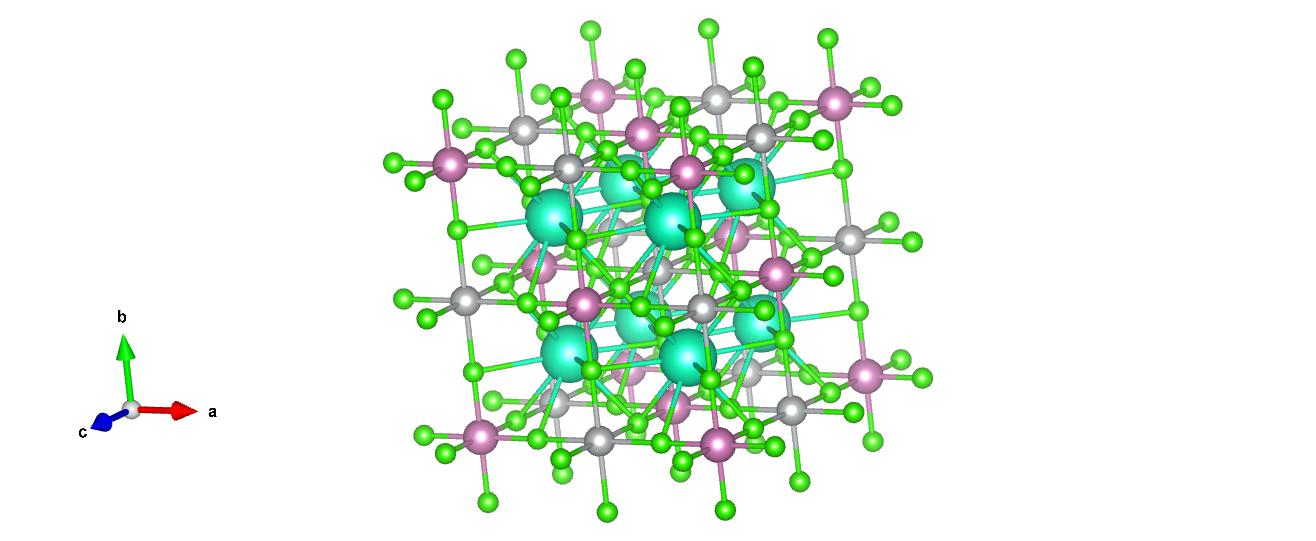
\includegraphics[width=1\textwidth]{Cs2AgInCl6.jpg}
\caption{Structure Visualised in Vesta}
\end{figure}
\begin{enumerate}
    \item Cs: 12
    \item Ag: 6
    \item In: 6
\end{enumerate}

\subsection*{Part b) Bond Lengths}
The bond lengths were found using the bond length operator and was found to be:
\begin{enumerate}
    \item Cs-Cl: 3.707 {\AA}
    \item Ag-Cl: 2.733 {\AA}
    \item In-Cl: 2.507 {\AA}
\end{enumerate}

\subsection*{Part c) Hide bonds greater than 3\AA}
The Cs-Cl bond were greater than 3\AA. Those were removed and the resulting structure is as given below.
\begin{figure}[ht]
\centering
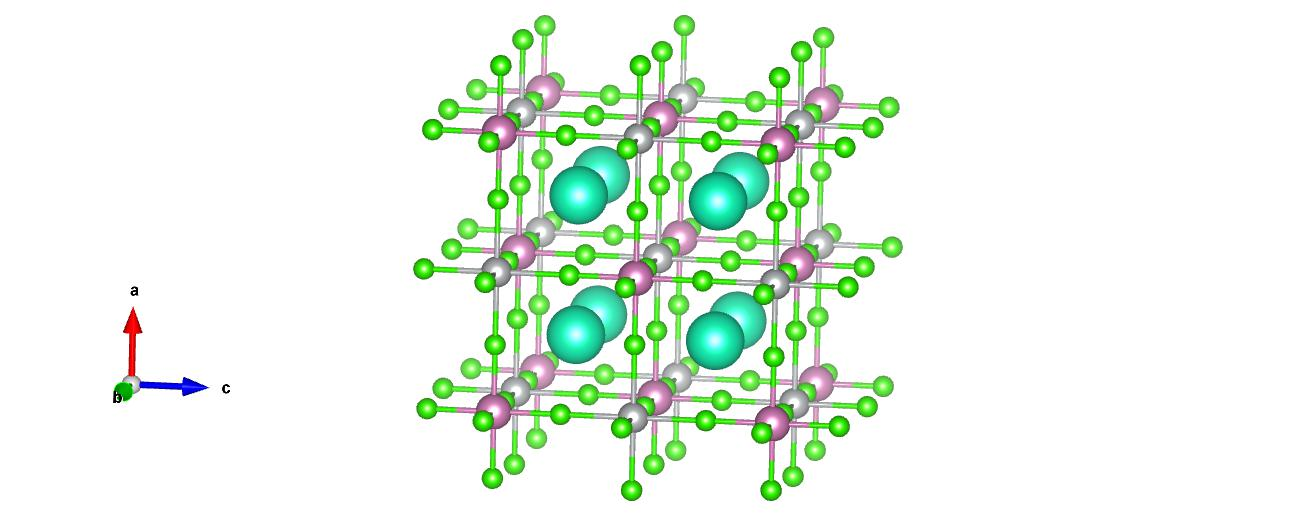
\includegraphics[width=1\textwidth]{part c.jpg}
\caption{Longer Bonds Removed}
\end{figure}

\subsection*{Part d) Polyhedral Mode}
\begin{figure}[ht]
\centering
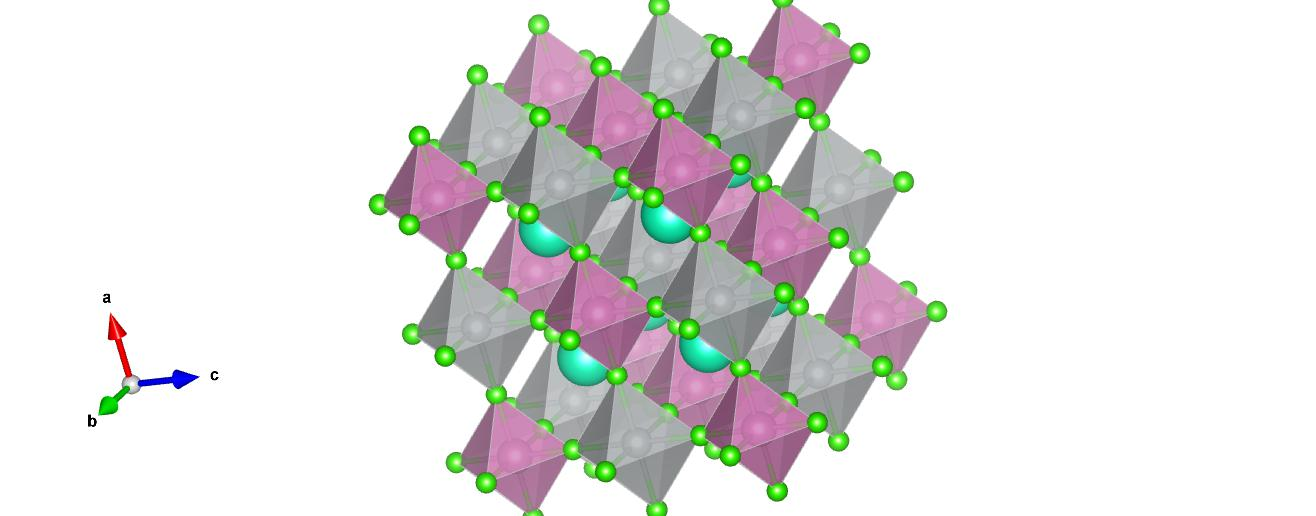
\includegraphics[width=1\textwidth]{part d) polyhedra.jpg}
\caption{Polyhedral Mode}
\end{figure}
Purple octahedra are constructed with In (Indium) atom as centre and grey octahedra are constructed with Ag (Silver) atom as centre 

\newpage
\subsection*{Part e) Pore Visualisation}
Cs atoms are hidden from the above structure
\begin{figure}[ht]
\centering
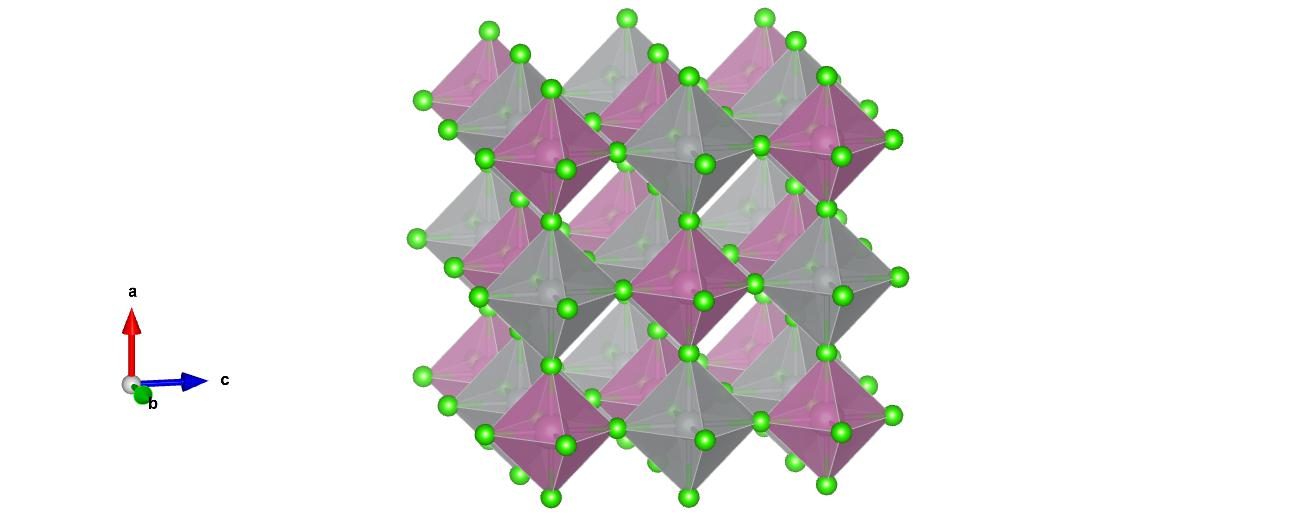
\includegraphics[width=1\textwidth]{part e.jpg}
\caption{Structure obtained after hiding the Cs atoms}
\end{figure}
\begin{figure}[ht]
\centering
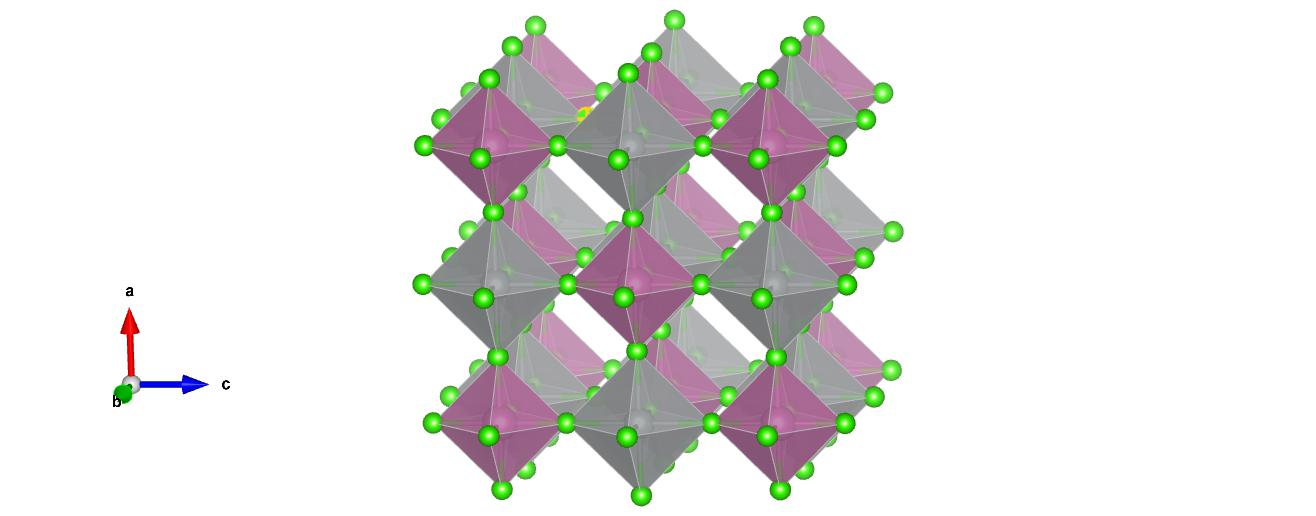
\includegraphics[width=1\textwidth]{part e backup.jpg}
\caption{Structure obtained after hiding the Cs atoms; with the narrow pores visible}
\end{figure}

\subsection*{Part f) Unit Cell \& Cation locations}
After hiding the bonds and polyhedra we obtain figure \ref{Unit Cell}. These are the coordinates of cations:
\begin{enumerate}
    \item Locations of \textbf{Ag} atoms (\textbf{13 atoms} in total displayed; 12 present in \textbf{edge centres} and 1 present in \textbf{body centre})
    \begin{enumerate}
        \item (10.48059,  0.00000,   5.24030)
        \item (0.00000,   0.00000,  5.24030)
        \item (0.00000,   10.48059, 5.24030)
        \item (10.48059,  10.48059, 5.24030)
        \item (0.0000,    5.2403,   0.00000)
        \item (0.0000,    5.2403,   10.48059)
        \item (10.48059,  5.24030,  10.48059)
        \item (10.48059,  5.24030,  0.0000)
        \item (5.24030,   0.00000,  10.48059)
        \item (5.24030,   10.48059, 0.0000)
        \item (5.24030,   0.00000,  0.00000)
        \item (5.24030,   10.48059, 10.48059)
        \item (5.24030,   5.24030,   5.24030)
    \end{enumerate}
    \item Locations of \textbf{In} atoms (\textbf{16 atoms} in total displayed; 6 present in \textbf{face centres} and 8 in \textbf{corners})
    \begin{enumerate}
        \item (0,0,0)
        \item (10.48059,  0.00000,   0.00000)
        \item (5.24030,   5.24030,   0.00000)
        \item (5.24030,  10.48059,   5.24030)
        \item (10.48059,   5.24030,   5.24030)
        \item (10.48059,   0.00000,  10.48059)
        \item (10.48059,  10.48059,   0.00000)
        \item (10.48059,  10.48059,  10.48059)
        \item (10.48059,   0.00000,  10.48059)
        \item (5.24030,   5.24030,  10.48059)
        \item (0.00000,   0.00000,  10.48059)
        \item (0.00000,  10.48059,  10.48059)
        \item (0.00000,   5.24030,   5.24030)
        \item (0.00000,  10.48059,   0.00000)
        \item (5.24030,  10.48059,   5.24030)
        \item (5.24030,   0.00000,   5.24030)
    \end{enumerate}
    \item Locations of \textbf{Cs} atoms (\textbf{8 atoms} in total displayed; All of them present in \textbf{tetrahedral voids})
    \begin{enumerate}
        \item (2.62015,   2.62015,   2.62015)
        \item (7.86044,   2.62015,   2.62015)
        \item (2.62015,   7.86044,   2.62015)
        \item (2.62015,   2.62015,   7.86044)
        \item (2.62015,   7.86044,   7.86044)
        \item (7.86044,   7.86044,   2.62015)
        \item (7.86044,   2.62015,   7.86044)
        \item (7.86044,   7.86044,   7.86044)
    \end{enumerate}
\end{enumerate}
\begin{figure}[ht]
\centering
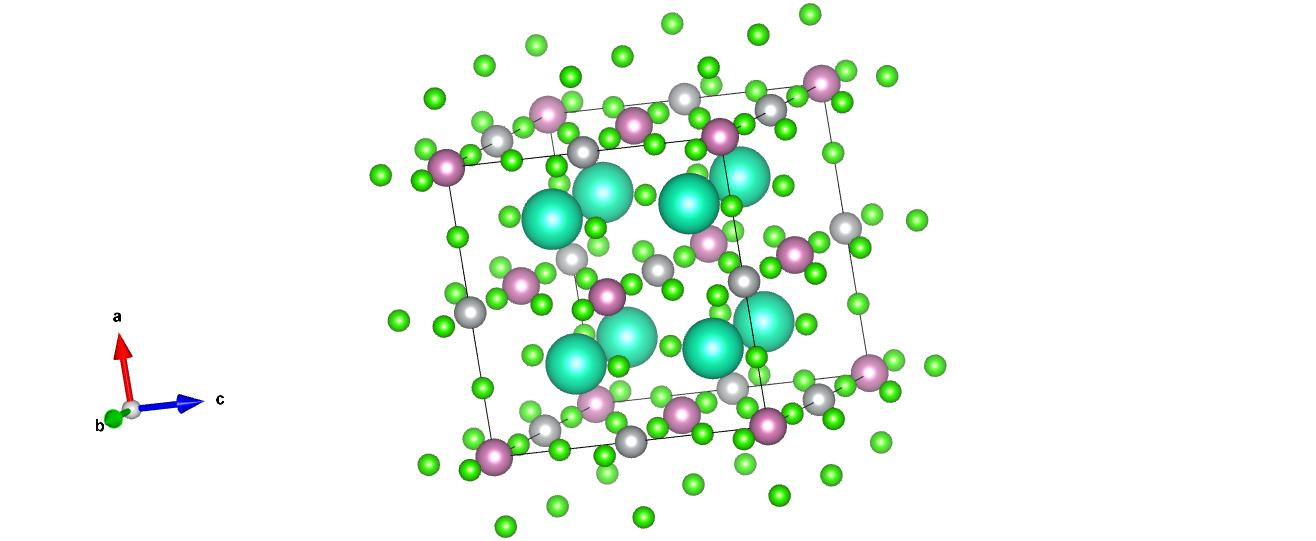
\includegraphics[width=1\textwidth]{part f).jpg}
\caption{Visualising the unit cell}
\label{Unit Cell}
\end{figure}
Effective number of Ag atoms = $12*\frac{1}{4} + 1 = 4$ \\
Effective number of Cs atoms = $8*1 = 8$ \\
Effective number of In atoms = $8*\frac{1}{8} + 6*\frac{1}{6} = 4$ \\
Effective number of Cl atoms = $48*\frac{1}{4} + 12*\frac{1}{2} = 24$\\
(48 atoms on edges in the middle of edge centre and corner. 12 atoms on faces in the middle of face centre and an edge centre)
\begin{figure}[ht]
\centering
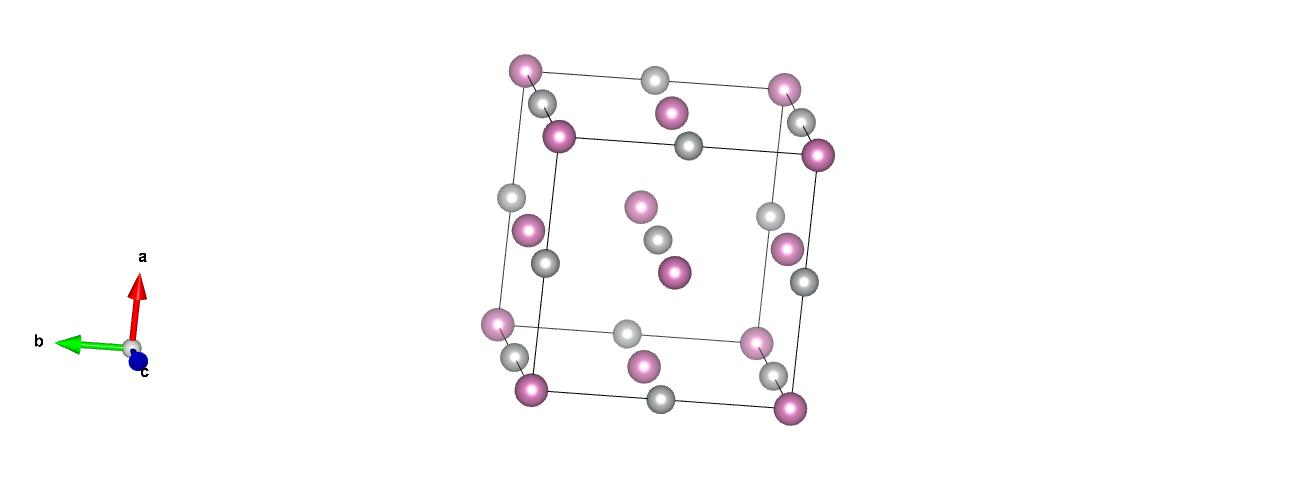
\includegraphics[width=1\textwidth]{q1part_f_cations.jpg}
\caption{Visualising the unit cell with just the cations}
\label{Cations}
\end{figure}


\subsection*{Part g) Miller Planes}

\begin{figure}[!htb]
\centering
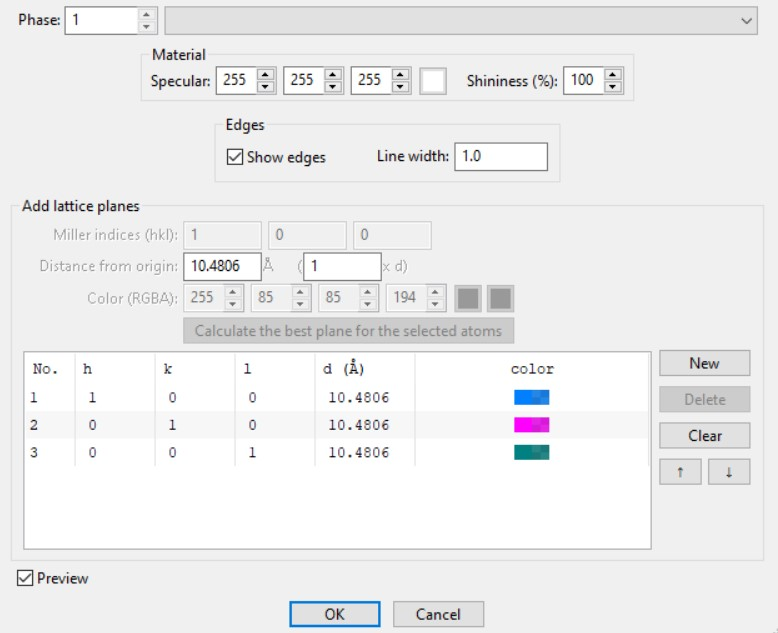
\includegraphics[width=1\textwidth]{part_g_key.jpg}
\caption{Generating the planes in Vesta}
\end{figure}

\begin{figure}[!htb]
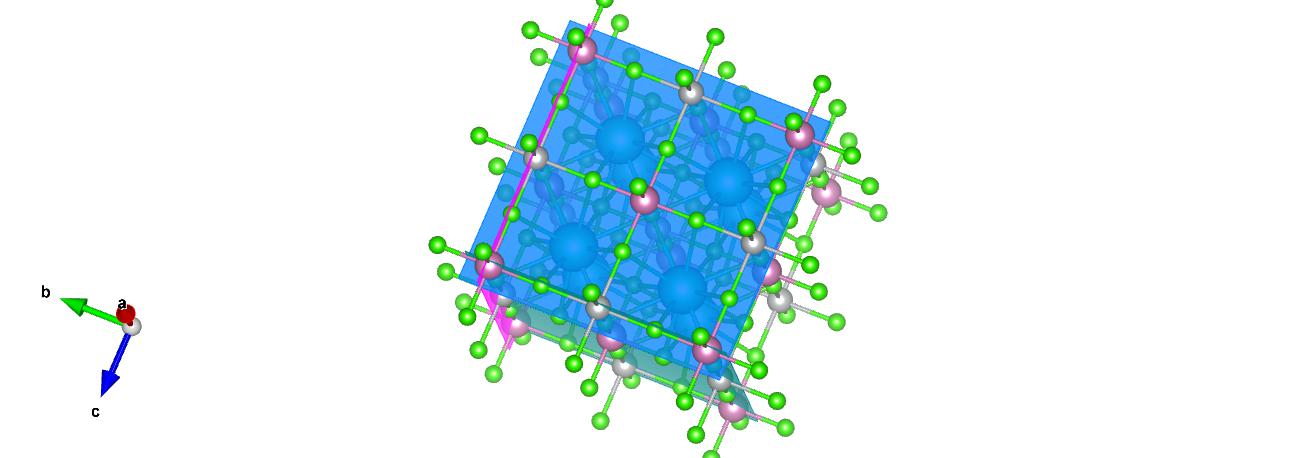
\includegraphics[width=0.75\textwidth]{q1part_g1.jpg}
\caption{Plane (100)}
\end{figure}
\FloatBarrier

\begin{figure}[ht]
\centering
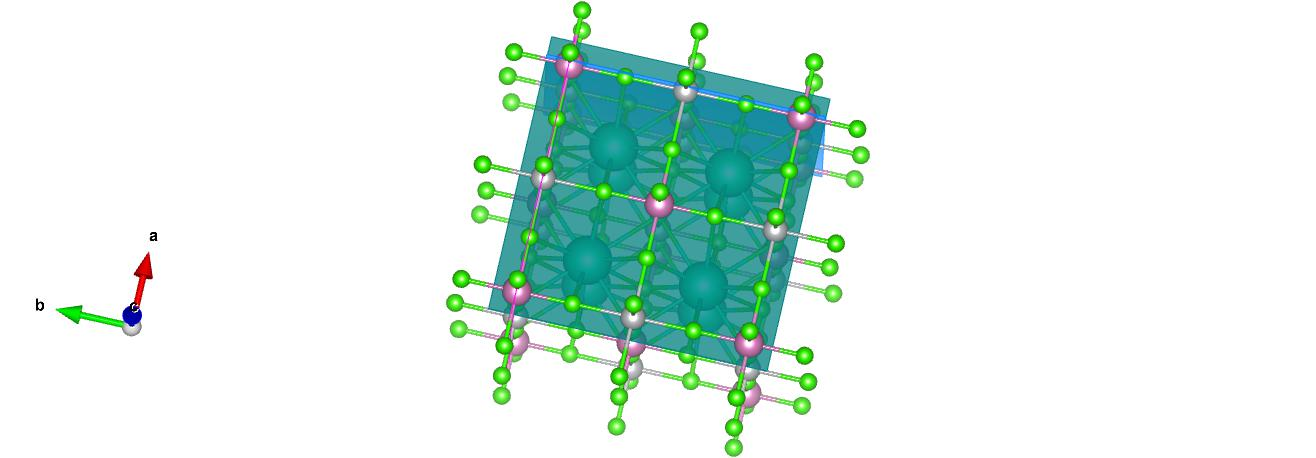
\includegraphics[width=1\textwidth]{q1part_g2.jpg}
\caption{Plane (001)}
\end{figure}
\FloatBarrier

\begin{figure}[ht]
\centering
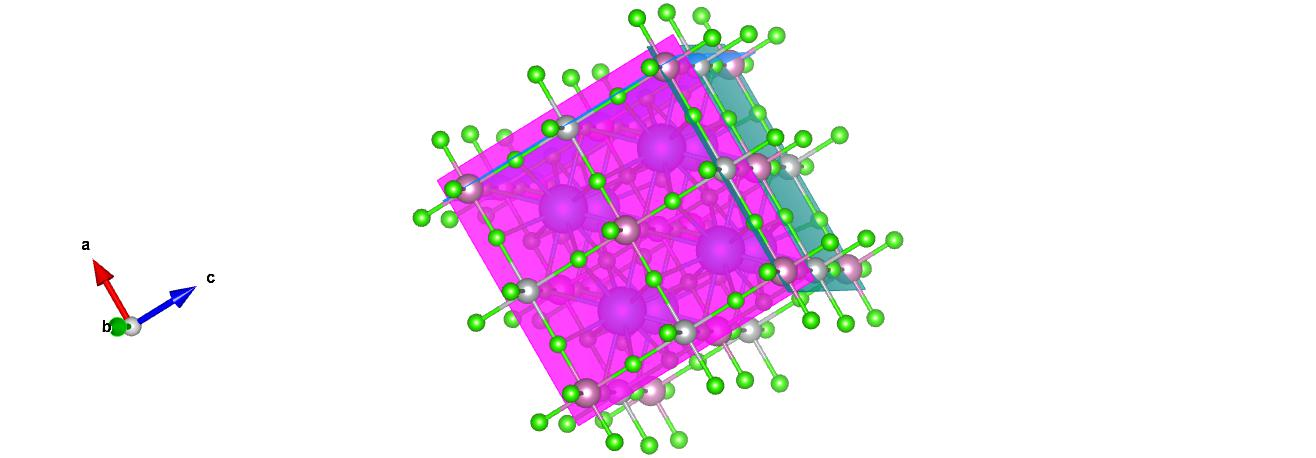
\includegraphics[width=1\textwidth]{q1part_g3.jpg}
\caption{Plane (010)}
\end{figure}
\FloatBarrier

\textbf{Yes}, all planes have the \textbf{same atom composition}: In in corners and centre. Silver in edge centres. Chlorine atoms in between In and Ag parallel to edges.
All the planes belong to the \textbf{same family}.


\subsection*{Part h) Family of Planes}

\begin{figure}[ht]
\centering
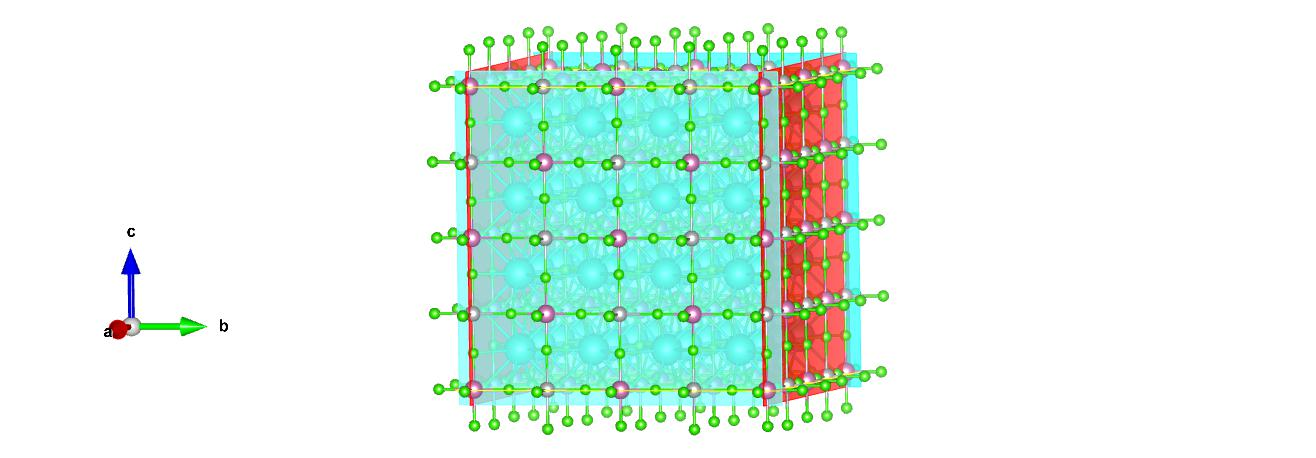
\includegraphics[width=0.75\textwidth]{q1part_h1.jpg}
\caption{(100) Plane}
\end{figure}

\begin{figure}[ht]
\centering
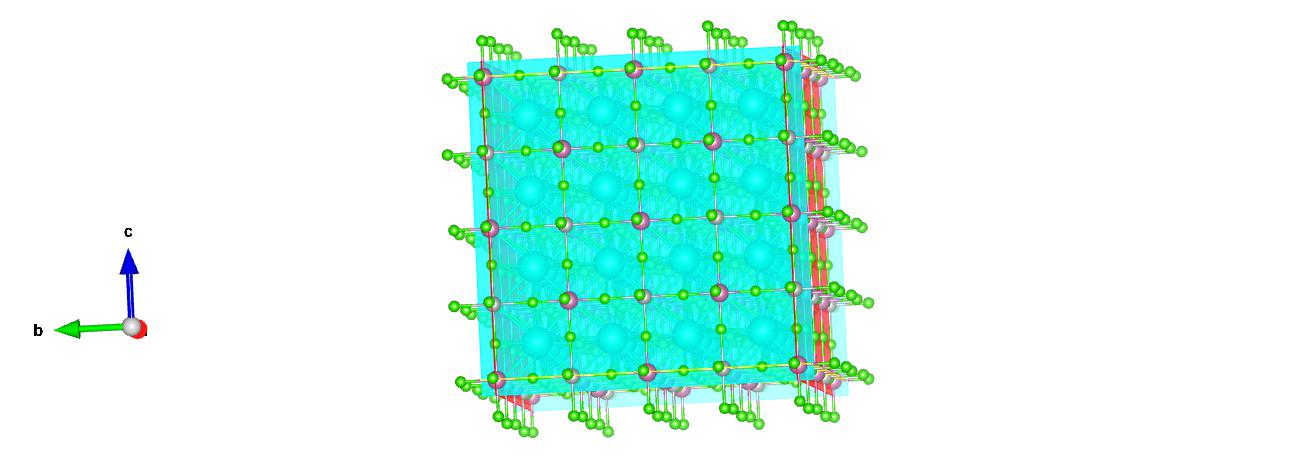
\includegraphics[width=0.75\textwidth]{q1part_h2.jpg}
\caption{(-100) Plane}
\end{figure}

\begin{figure}[ht]
\centering
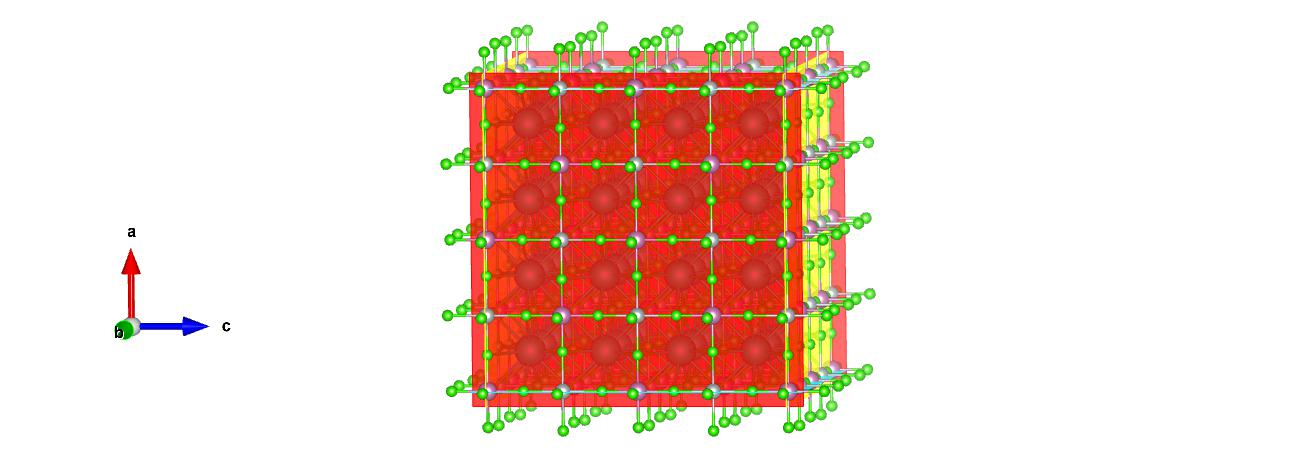
\includegraphics[width=0.75\textwidth]{q1part_h3.jpg}
\caption{(010) Plane}
\end{figure}

\begin{figure}[ht]
\centering
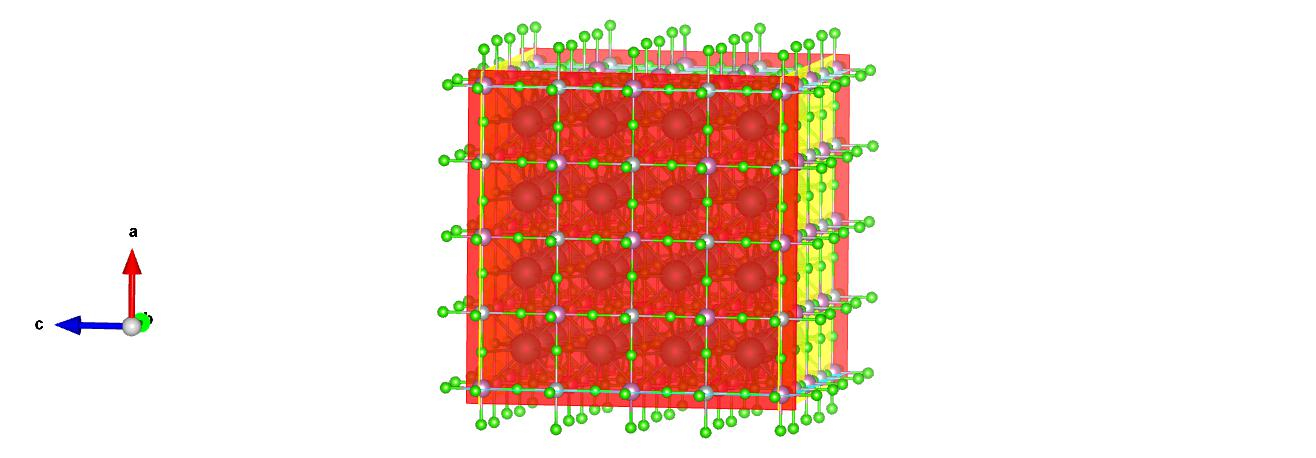
\includegraphics[width=1\textwidth]{q1part_h4.jpg}
\caption{(0 -1 0) Plane}
\end{figure}

\begin{figure}[ht]
\centering
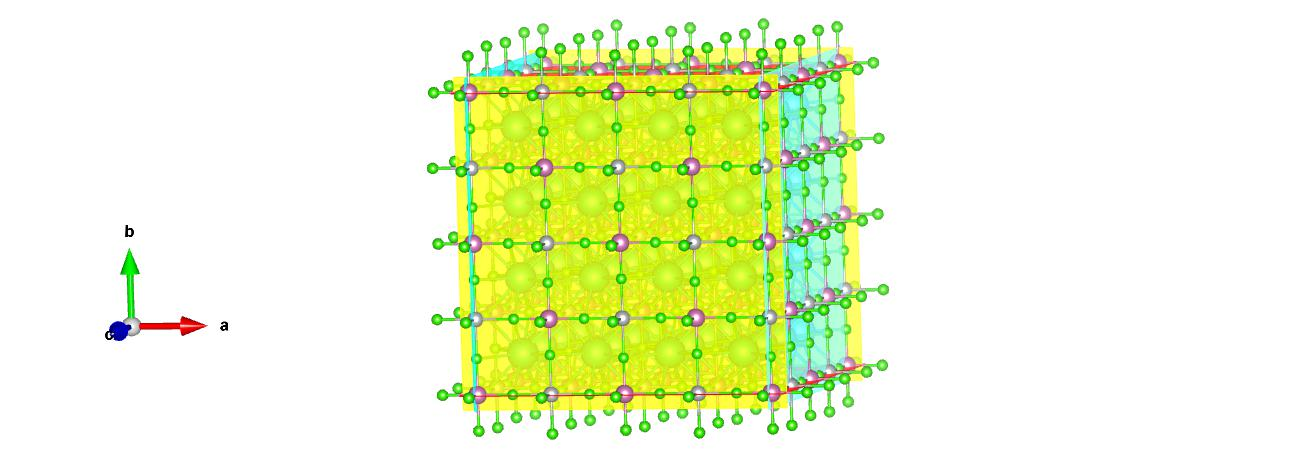
\includegraphics[width=1\textwidth]{q1part_h5.jpg}
\caption{(001) Plane}
\end{figure}

\begin{figure}[ht]
\centering
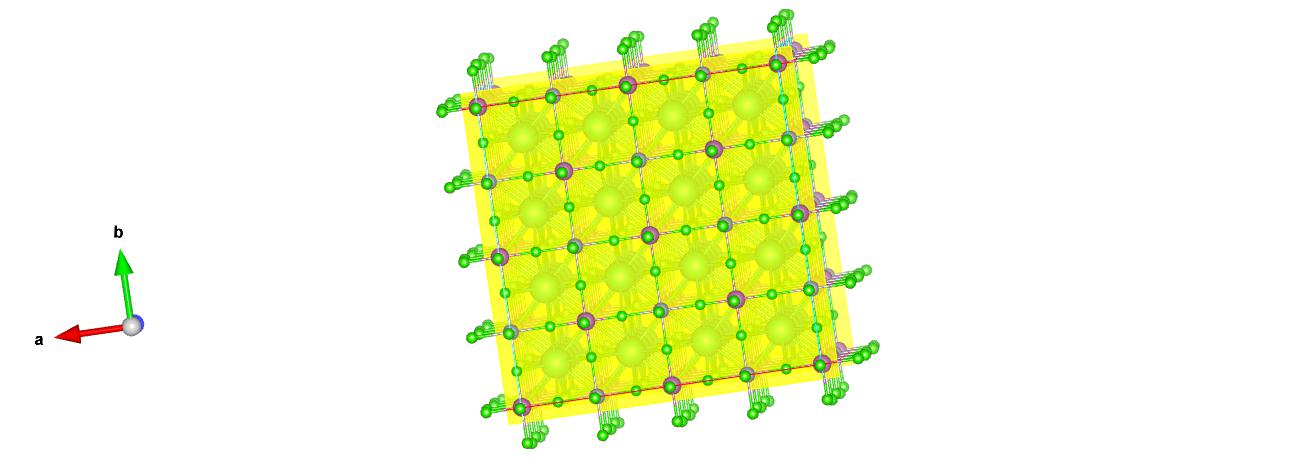
\includegraphics[width=1\textwidth]{q1part_h6.jpg}
\caption{(0 0 -1) Plane}
\end{figure}
\FloatBarrier


\subsection*{Part i) Comparing (101) and (100) planes}
\textbf{100 Plane} (Refer figure \ref{100}) \\
Bond Lengths:
\begin{enumerate}
    \item In-Cl: 2.507\AA
    \item Ag-Cl: 2.733\AA
\end{enumerate}
Bond Angles:
\begin{enumerate}
    \item Cl-Ag-Cl: $90^{\circ}$
    \item Cl-In-Cl: $90^{\circ}$
\end{enumerate}
\textbf{101 Plane} (Refer figure \ref{101}) \\
Bond Lengths:
\begin{enumerate}
    \item In-Cl: 2.507\AA
    \item Ag-Cl: 2.733\AA
    \item Cs-Cl: 3.7072\AA
\end{enumerate}
Bond Angles:
\begin{enumerate}
    \item Cl-Ag-Cl: $90^{\circ}$
    \item Cl-In-Cl: $90^{\circ}$
    \item Cl-Cs-Cl: $62.84^{\circ}$
\end{enumerate}
Between the same set of atoms, bond angles and bond lengths remain the same across planes.
\begin{figure}[ht]
\centering
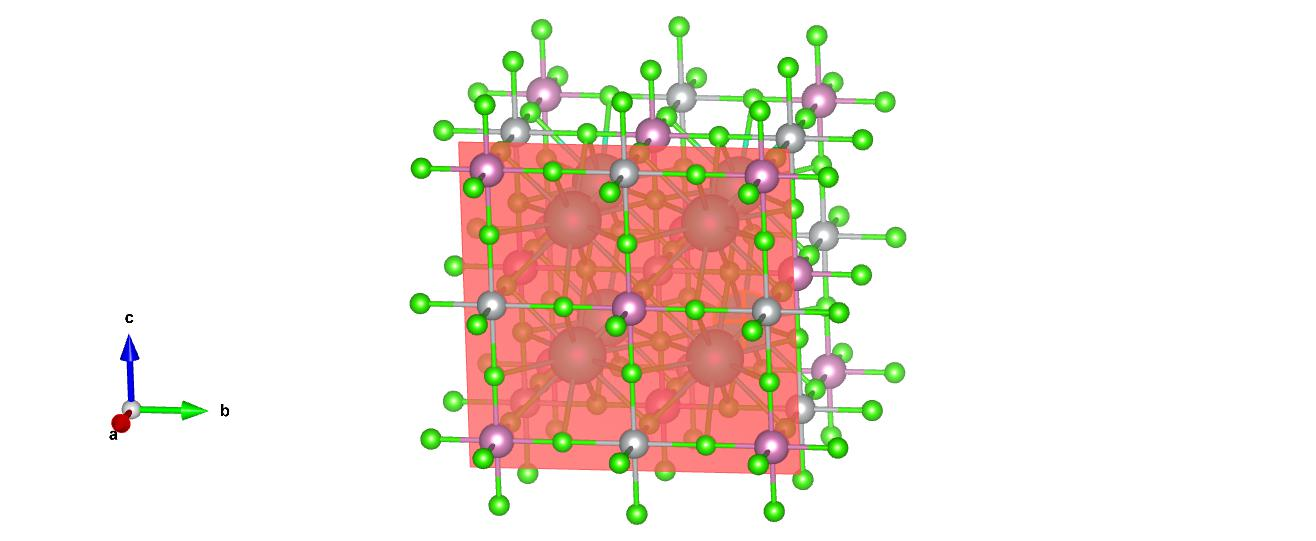
\includegraphics[width=1\textwidth]{q1part_i_100.jpg}
\caption{Atoms on 100 Plane}
\label{100}
\end{figure}
\FloatBarrier
\begin{figure}[!h]
\centering
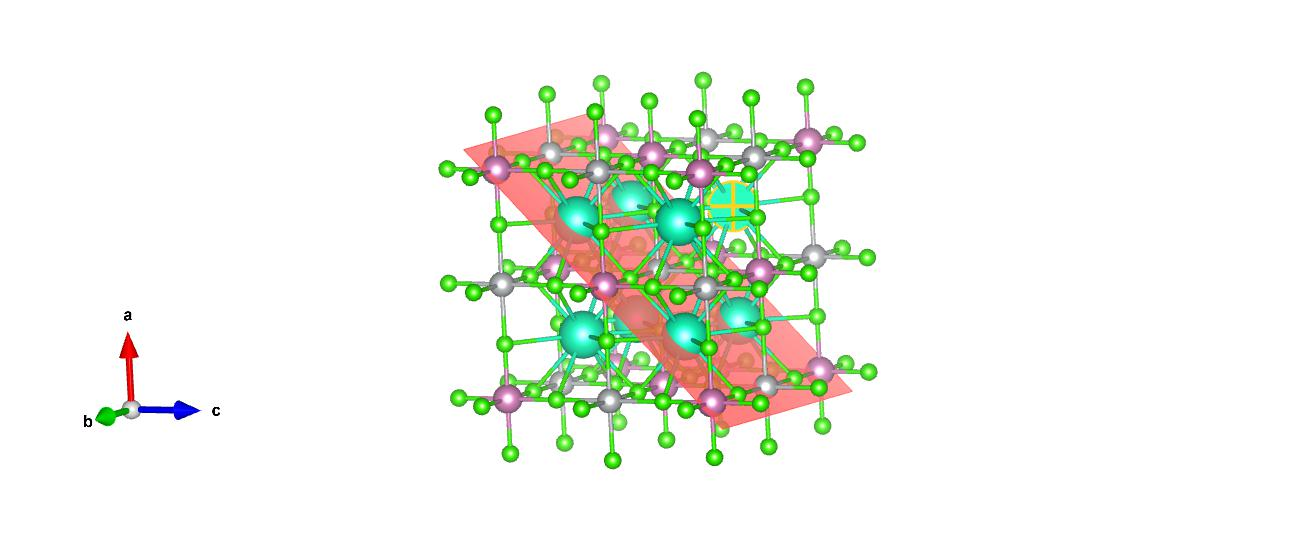
\includegraphics[width=1\textwidth]{q1part_i_101.jpg}
\caption{Atoms on 101 Plane}
\label{101}
\end{figure}
\FloatBarrier

\exercise
\subsection*{Part a)}
Given below is an extract of the lines mentioning the cell parameters in the CIF file:
\begin{lstlisting}
_cell_length_a  10.480593(54)
_cell_length_b  10.480593(54)
_cell_length_c  10.480593(54)
_cell_angle_alpha 90
_cell_angle_beta  90
_cell_angle_gamma 90
_cell_volume 1151.218(18)
\end{lstlisting}
From the above lines in the \textit{.CIF} file we find that the parameter values are $a = b = c = 10.4806$\AA{}  and $\alpha = \beta = \gamma = 90^{\circ}$
\\
Parameters as shown in Vesta:
\begin{figure}[!h]
\centering
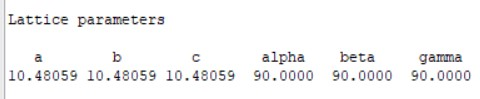
\includegraphics[width=1\textwidth]{vesta_params.jpg}
\caption{Screenshot of parameters displayed in Vesta}
\end{figure}
\FloatBarrier
Obviously, since Vesta takes the parameters from the CIF file, the parameters taken in both places match perfectly.
\\
\textbf{Space Group: Fm-3m} \tab \textbf{Space Group Number: 225}
\\
\underline{Explanation}:
\begin{enumerate}
    \item \textbf{F}: It gives the crystal system and centering. The structure is \textbf{Face Centred Cubic}
    \item The first \textbf{m} denotes that there is mirror symmetry with mirror placed along a-axis.
    \item \textbf{-3} denotes that there is an inversion symmetry and a $C_3$ rotational symmetry with respect to b-axis.
    \item The final \textbf{m} denotes that there is a mirror symmetry with mirror along c-axis
\end{enumerate}

\subsection*{Part b) Symmetry Operations}
Space Group Number was found to be \textbf{225} from this  \href{http://img.chem.ucl.ac.uk/sgp/large/sgp.htm}{link}.
\\
Space Group Diagram was obtained in the following \href{http://img.chem.ucl.ac.uk/sgp/large/225az1.htm}{link}.
\begin{figure}[!h]
\centering
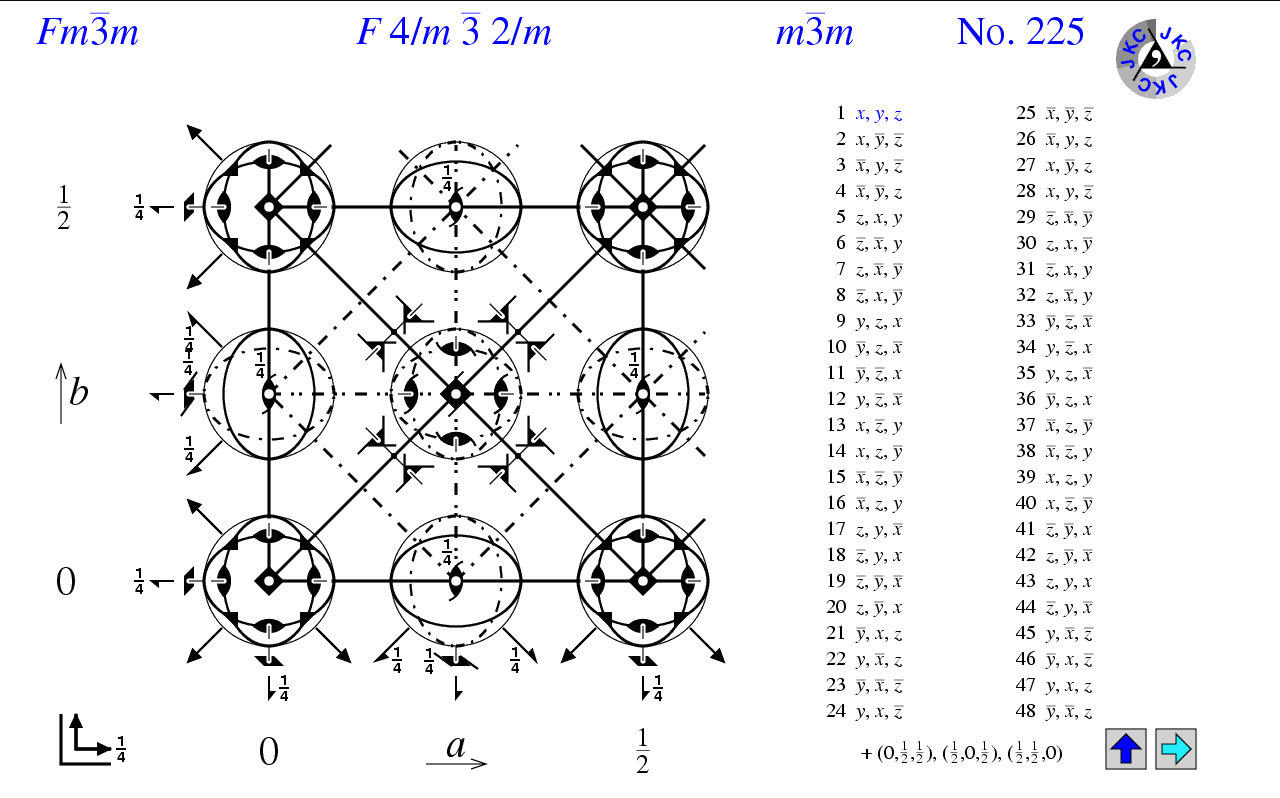
\includegraphics[width=1\textwidth]{space_group_diagram.png}
\caption{Space group diagram of $Cs_{2}AgInCl_{6}$}
\end{figure}
\FloatBarrier
We find that the crystal has the following symmetry operations:
\begin{enumerate}
    \item $3_1$ screw axis inclined to plane at an angle of $54.736^{\circ}$.
    \item $3_2$ screw axis inclined to plane at an angle of $54.736^{\circ}$.
    \item $2_1$ screw axis perpendicular to the plane of the screen with inversion on the axis. The inversion centre lies at a height of 1/4 lattice units.
    \item $2_1$ screw axis inclined to the plane at an angle of $45^{\circ}$
    \item $2_1$ screw axis parallel to the plane
    \item Glide plane along the diagonals.
    \item $4_2$ screw axis perpendicular to the plane with centre of inversion on the axis.
    \item $4_2$ screw axis along '-a' and '-b' directions(parallel to plane), with height of the axis of rotation above the XY plane at $\frac{1}{4}$.
    \item $C_4$ symmetry with respect to axis perpendicular to the plane with a centre of inversion on the axis.
    \item $C_4$ symmetry with respect to axis along '-a' and '-b' directions.(parallel to plane)
    \item $C_2$ symmetry with respect to axes along and opposite to 'a' and 'b' directions. (parallel to the plane)
    \item Diagonal planes:
    \begin{enumerate}
        \item Inclined at $45^{\circ}$ to the plane.
        \item The dashed-dotted line (which bisects the -YZ axes) indicates a glide direction simultaneously along X and -YZ (look at the spheres in edge centres)
        \item The thick solid line shows a mirror plane bisecting the YZ axes, i.e. with its normal parallel to -YZ. (look at the spheres in corners)
    \end{enumerate} 
    
\end{enumerate}
\end{document}